\begin{flushleft}
Lo script usato è il seguente:
\lstinputlisting[language=MatLab]{cap_2/es7/es7.m}
Il numero di iterazioni del metodo di bisezione risultanti sono:

\begin{center}
\begin{tabular}{|c|c|c|c|}
\hline
$tol_x$ & bisezione \\
\hline
$10^{-1}$ & 2 \\
$10^{-2}$ & 7 \\
$10^{-3}$ & 10 \\
$10^{-4}$ & 14 \\
$10^{-5}$ & 17 \\
$10^{-6}$ & 20 \\
$10^{-7}$ & 24 \\
$10^{-8}$ & 27 \\
$10^{-9}$ & 30 \\
$10^{-10}$ & 34 \\
\hline
\end{tabular}
\end{center}

Si può vedere dal grafico l'andamento dei vari metodi usati nel seguente plot MatLab:
\begin{figure}[H]
\label{fes27}
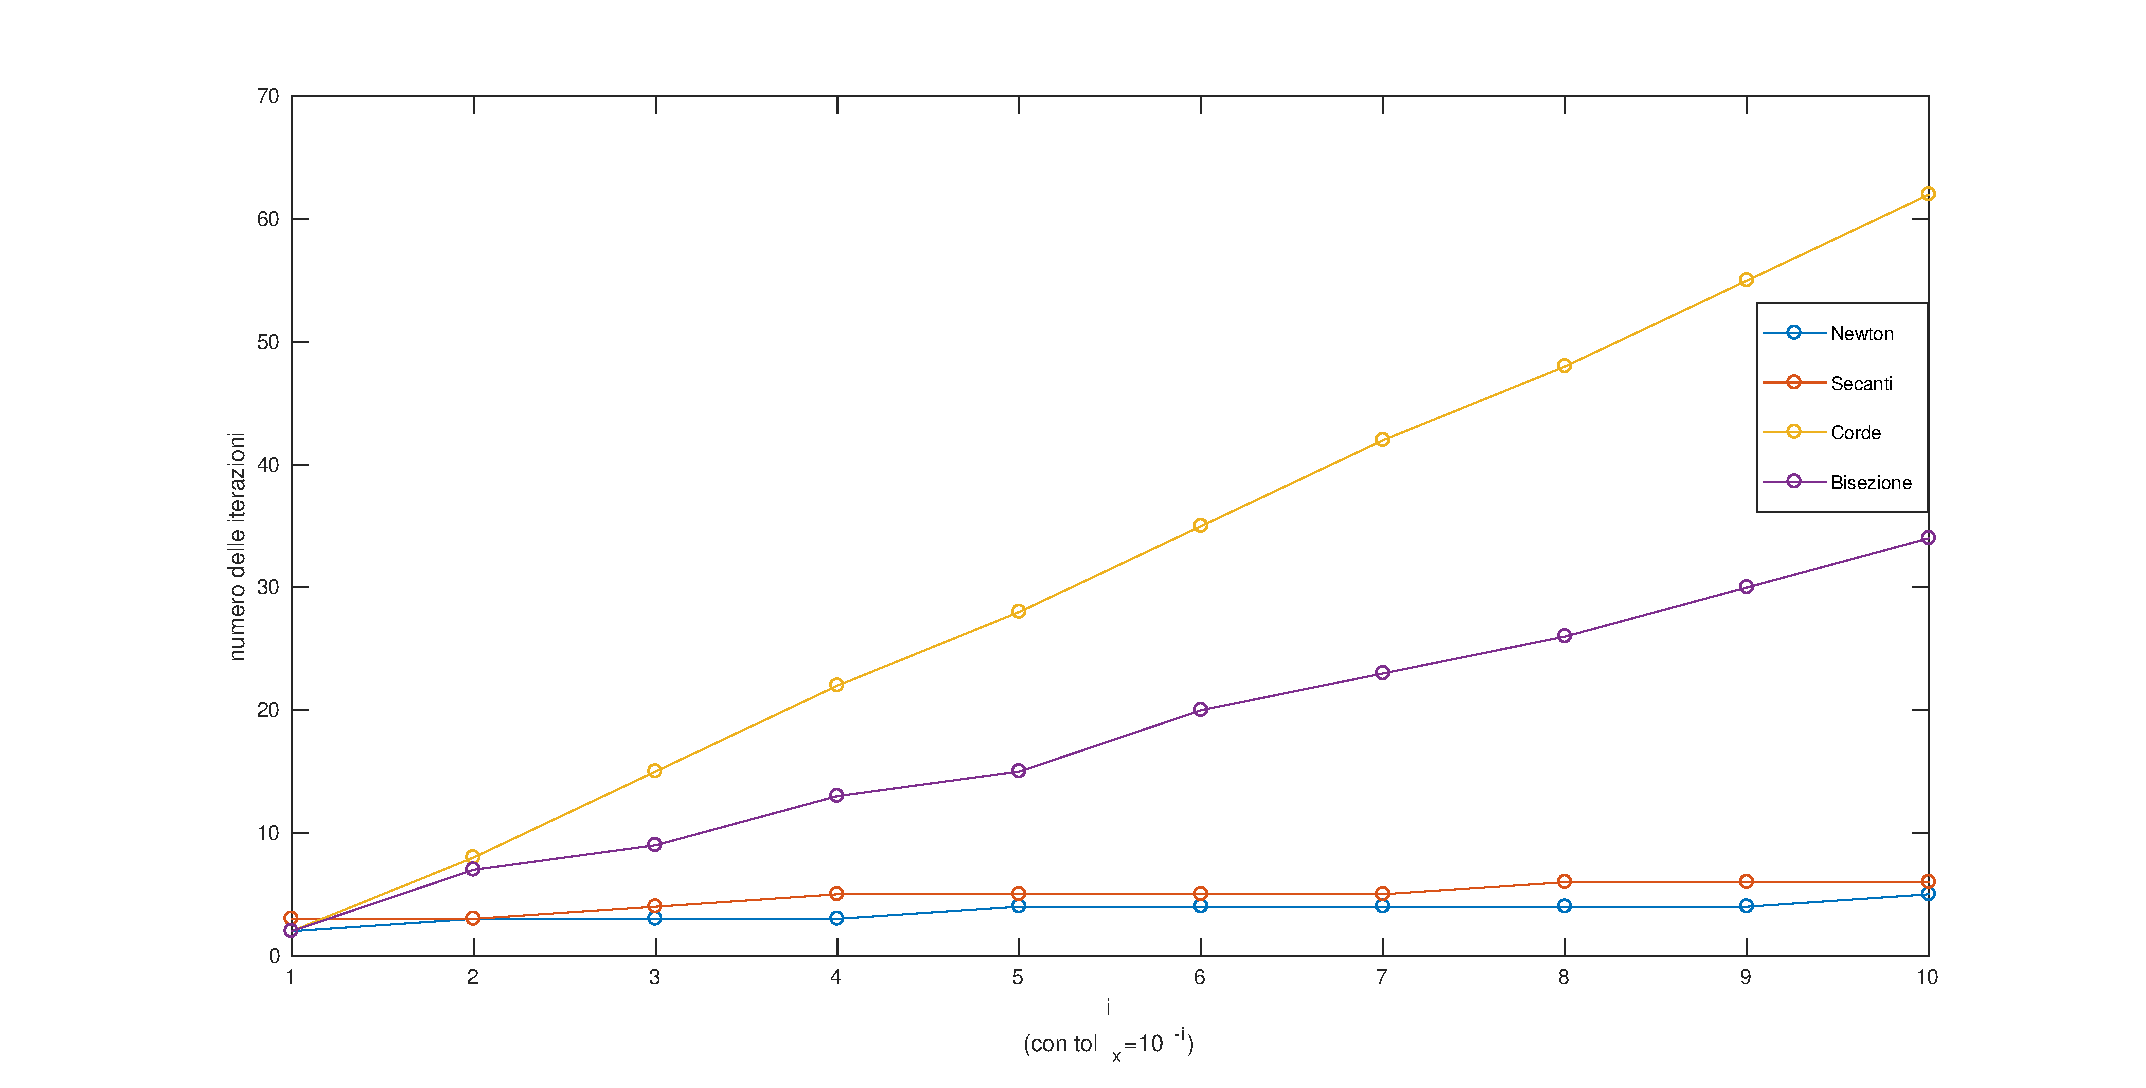
\includegraphics[width=480px, height=280px]{plot/fes27}
\caption{\texttt{Aggiunta dell'andamento del metodo di Bisezione rispetto ai precedenti metodi}}
\end{figure}

\end{flushleft}